% %% %%%%%%%%%%%%%%%%%%%%%%%%%%%%%%%%%%%%%%%%%%%%%%%%%%%%%%%%%%
% intro.tex
%
% Author:  Mauricio Matamoros
% License: MIT
%
% %% %%%%%%%%%%%%%%%%%%%%%%%%%%%%%%%%%%%%%%%%%%%%%%%%%%%%%%%%%%
%!TEX root = ../practica.tex
%!TEX root = ../references.bib

% CHKTEX-FILE 1
% CHKTEX-FILE 13
% CHKTEX-FILE 46

\section{Introducción}%
\label{seq:introduction}
La presente práctica resume los pasos a seguir para modular la cantidad de corriente que pasa por un foco incandescente con un microcontrolador.
En particular, se interesa en el uso de un circuito de detección de cruce por cero para conmutar un triac acoplado a un microcontrolador RP2040 utilizando MicroPython.
Los datos registrados serán posteriormente enviados vía \IIC a una Raspberry Pi para controlar la intencidad del foco.

% %% %%%%%%%%%%%%%%%%%%%%%%%%%%%%%%%%%%%%%%%%%%%%%%%%%%%%%%%%%%
% intro-bridge.tex
%
% Author:  Mauricio Matamoros
% License: MIT
%
% %% %%%%%%%%%%%%%%%%%%%%%%%%%%%%%%%%%%%%%%%%%%%%%%%%%%%%%%%%%%
%!TEX root = ../practica.tex
%!TEX root = ../references.bib

% CHKTEX-FILE 1
% CHKTEX-FILE 13
% CHKTEX-FILE 46

\subsection{El puente rectificador}%
\label{seq:intro-bridge}

\begin{wrapfigure}{r}{0.3\columnwidth}
	\centering
	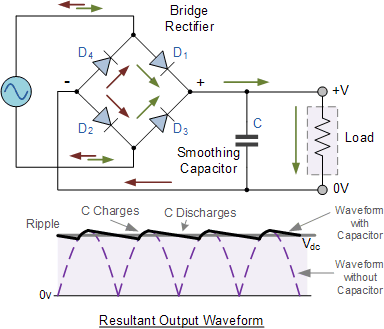
\includegraphics[width=0.3\columnwidth]{img/bridge.png}
	\caption[Rectificador de onda completa]{Rectificador de onda completa\footnotemark{}}%
	\label{fig:bridge}
\end{wrapfigure}
\footnotetext{Fuente de imagen: \url{https://lasopaeden528.weebly.com/bridge-rectifier-calculator.html}}
Un puente rectificador o rectificador de onda completa es un arreglo de 4 diodos que permiten el paso de la corriente en un sólo sentido, invirtiendo así la parte negativa de una señal de AC respecto a su voltaje de referencia.
Los puentes rectificadores son un componente fundamental en los transformadores de corriente de AC a DC.

El circuito funciona de la siguiente manera.
En la primera parte del ciclo, cuando el voltaje comienza a aumentar, la corriente fluye de la parte norte del puente (arriba) a través de $D_1$ hacia la carga, y luego de regreso por $D_2$ hacia el neutro (véase~\Cref{fig:bridge}).
En esta primera etapa, $D_3$ y $D_4$ actuan como barreras evitando que la corriente fluya directamente de la fase al neutro (corto circuito).
Tras pasar por la carga, el voltaje en en el ánodo de $D_4$ ha caído y es menor que en el cátodo, por lo que no habrá flujo de corriente en esta dirección, pero aún es positivo respecto al neutro ($V_{N}=0$), por lo que la corriente tendrpa que pasar por $D_1$.
De forma análoga, el voltaje en el cátodo de $D_3$ es menor que en el ánodo, por lo que tampoco habrá flujo en esta dirección.

En la segunda parte del ciclo, el voltaje de fase disminuye respecto al neutro, por lo que la corriente fluye de la parte sur del puente (abajo) a través de $D_3$ hacia la carga, y luego de regreso por $D_4$ hacia la fase (véase~\Cref{fig:bridge}).
En esta segunda etapa, $D_1$ y $D_2$ actuan como barreras evitando que la corriente fluya directamente del neutro a la fase (corto circuito).
Tras pasar por la carga, el voltaje en en el ánodo de $D_2$ ha caído y es menor que en el cátodo, por lo que no habrá flujo de corriente en esta dirección, pero aún es positivo respecto a la fase ($V_{N}=0$), por lo que la corriente tendrpa que pasar por $D_4$.
De forma análoga, el voltaje en el cátodo de $D_1$ es menor que en el ánodo, por lo que tampoco habrá flujo en esta dirección.

% %% %%%%%%%%%%%%%%%%%%%%%%%%%%%%%%%%%%%%%%%%%%%%%%%%%%%%%%%%%%
% intro-opto.tex
%
% Author:  Mauricio Matamoros
% License: MIT
%
% %% %%%%%%%%%%%%%%%%%%%%%%%%%%%%%%%%%%%%%%%%%%%%%%%%%%%%%%%%%%
%!TEX root = ../practica.tex
%!TEX root = ../references.bib

% CHKTEX-FILE 1
% CHKTEX-FILE 13
% CHKTEX-FILE 46

\subsection{Optoacopladores}%
\label{seq:intro-opto}
Un optoacoplador o optoaislador es un circuito integrado que permite aislar mecánicamente dos circuitos, por lo que se usa comunmente para separar la lógica de control de los circuitos de potencia.
El principio básico de un optoacoplador, como su nombre lo indica, es utilizar transductores ópticos para la transmisión de señales eléctricas.
Así, en un lado del optoacoplador se tendrá siempre un diodo LED y en el otro extremo un fotoreceptor, que puede ser un foto SRC, un foto dárlington, un foto TRIAC o un fototransistor, siendo este último el más común.

En un optoacoplador, el diodo LED emite una cantidad de luz directamente proporcional a la corriente que circula por éste y, al incidir ésta en el fotoreceptor, el estímulo luminoso activa el paso de corriente a través de éste.
Por ejemplo, en el caso de un fototransistor, al incidir la luz en la juntura de la base ésta se ioniza, generando un puente de iones que permite el flujo entre los extremos del transistor.
Además, la mayoría de los optoacopladores tienen un pin conectado directamente a la base que sirve para ajustar la sensibilidad de la misma mediante la inyección de un voltaje pequeño.

Los fototransistores foto-dárlingtons se utilizan principalmente en circuitos DC, mientras que los foto SCR y los foto TRIACs permiten controlar los circuitos de AC.
Existen muchos otros tipos de combinaciones de fuente-sensor tales como LED-fotodiodo, LED-LÁSER, pares de lámpara-fotorresistencia, optoacopladores reflectantes y ranurados.

Por ejemplo, el integrado 4N25 puede usarse para monitorear el voltaje de la línea de tensión doméstica con un integrado.
Según su hoja de especificaciones~\Citep{4N25datasheet}, la entrada del 4N25 acepta hasta 60mA, permite un flujo por el colector de hasta 50mA, y aisla hasta 5000V\textsubscript{RMS}.
Si se toma como entrada un voltaje de línea rectificado de 127V\textsubscript{RMS} y se limita la corriente a la corriente de prueba de 50mA indicada en la hoja de especificaciones~\Citep{4N25datasheet}, el 4N25 tendrá que acoplarse con una resistencia de al menos 2K7$\Omega$ aproximada mediante la fórmula:

\begin{equation*}
R=\frac{V}{I}=\frac{127V_\text{RMS}}{0.050A}
= 2540\Omega
\end{equation*}

Sin embargo, como $P=I^2R$ una resistencia de 2k7$\Omega$ disiparía ${\left(47mA\right)}^{2}\times 2.7k\Omega = 5.96\text{Watt}$, que es un tremendo desperdicio de energía disipada como calor.

En este caso conviene reducir mucho más la corriente que circula por el 4N25.
Supóngase que el propósito del 4N25 fuera el de activar una interrupción en un microcontrolador.
Normalmente las entradas digitales de los microcontroladores requieren de unos cuantos microamperios para activarse, por lo que pueden elegirse $10\mu A$ como un valor conservador seguro.
Por otro lado, la hoja de especificaciones nos indica que la corriente que circula por el transistor será el 50\% de la corriente que pase por el fotodiodo~\Citep{4N25datasheet}; por lo que la resistencia elegida tendrá que limitar la corriente a por lo menos $20\mu A$, en este caso:

\begin{equation*}
R=\frac{V}{I}=\frac{127V_\text{RMS}}{20\times{10}^{-6}A}
= 6350000\Omega \approx 5\text{M}6\Omega
\end{equation*}

Otro enfoque es considerar las resistencias comerciales más económicas en el mercado, es decir las de $\sfrac{1}{4}$Watt.
Como $P=\frac{V^2}{R}=0.25\text{Watt}$ y $V=127V$ entonces
\(
	R_\text{Max}
		=\frac{{\left(127V\right)}^2}{0.25\text{Watt}}
		=\frac{16129{V}^2}{0.25\text{Watt}}
		=64516\Omega \approx 68\text{K}\Omega
\)
cualquier resistencia de $68\text{K}\Omega$ o mayor será suficientemente grande para optoacoplar un microcontrolador a una línea de tensión de 127VAC con un 4N25 sin disipar mucho calor, proporcionando un flujo por el fototransistor de 0.9mA; más que suficiente para drenar un pin digital acoplado a \textsc{Vcc} con una resistencia de \emph{pull-up} de $10\text{K}\Omega$.

% %% %%%%%%%%%%%%%%%%%%%%%%%%%%%%%%%%%%%%%%%%%%%%%%%%%%%%%%%%%%
% intro-zerox.tex
%
% Author:  Mauricio Matamoros
% License: MIT
%
% %% %%%%%%%%%%%%%%%%%%%%%%%%%%%%%%%%%%%%%%%%%%%%%%%%%%%%%%%%%%
%!TEX root = ../practica.tex
%!TEX root = ../references.bib

% CHKTEX-FILE 1
% CHKTEX-FILE 13
% CHKTEX-FILE 46

\subsection{Detector de cruce por cero}%
\label{seq:intro-zeroX}
Un circuito detector de cruce por cero es un circuito electrónico diseñado para detectar cuando una señal senoidal pasa por cero.
Estos circuitos se usan comunmente en electrónica de potencia tanto para detectar la frecuencia de la línea y hacer cálculo de fases.
Además, al reducirse la diferencia de potencial a cero entre la fase y el neutro, la corriente instantánea también es cero, haciendo de éste el momento ideal para cortar la alimentación sin dañar las cargas.

\begin{figure}[H]
	\centering
	\begin{subfigure}[b]{0.5\columnwidth}
		\centering
		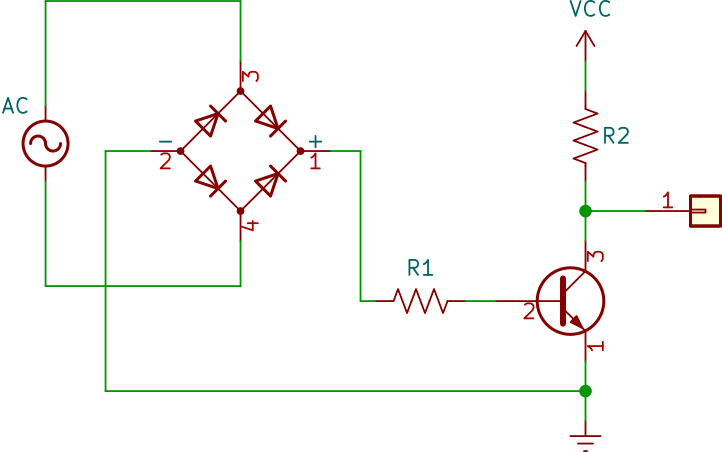
\includegraphics[width=\textwidth,height=5cm,keepaspectratio]{img/zcross-1.png}
		\caption{Detector de cruce por cero simple}
		\label{fig:zx1} %chktex 24
	\end{subfigure}%
	\begin{subfigure}[b]{0.5\columnwidth}
		\centering
		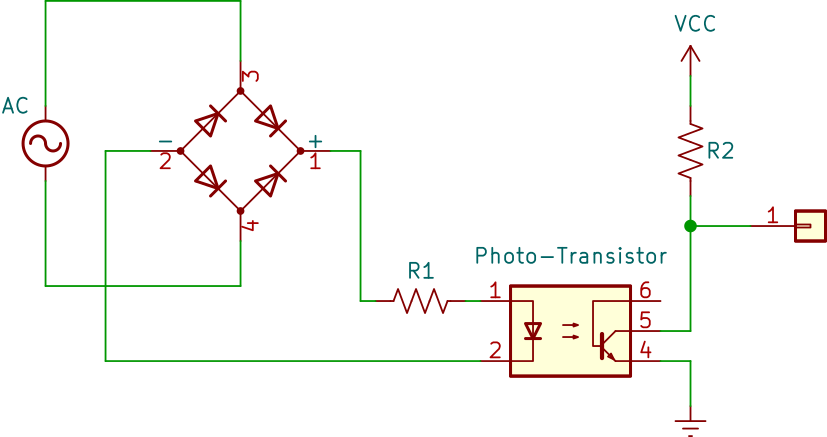
\includegraphics[width=\textwidth,height=5cm,keepaspectratio]{img/zcross-2.png}
		\caption{Detector de cruce por cero optoacoplado}
		\label{fig:zx2} %chktex 24
	\end{subfigure}
	\caption{Detectores de cruce por cero}
	\label{fig:zx} % chktex 24
\end{figure}

La forma más sencilla de alambrar un circuito detector de cruce por cero es mediante un puente rectificador, dos resistencias y un transistor tipo NPN en modo interruptor (véase~\Cref{fig:zx1}).
El puente rectificador se encarga de invertir la parte negativa de la señal de AC, evitando así corrientes inversas que el transistor es incapaz de manejar.
Cuando hay voltaje en la línea, éste habilita la base cerrando el circuito del transistor y conectando el pin de sensado a tierra (la resistencia de base evita el corto circuito y ajusta el umbral de sensibilidad).
Tan pronto como la diferencia de potencial entre la línea y el neutro cae a cero (o suficientemente bajo como la resistencia de base permita) el circuito se abre y en el pin de sensado se registra \textsc{Vcc}.

Para calcular $R_1$ es necesario tomar en cuenta las características eléctricas del transistor y los voltajes de pico de la línea.
Se sabe que $V_\text{pico}=V_\text{RMS}\sqrt{2}$, por lo que usando la ley de ohm se tiene:
\begin{equation}
	R_1 = \frac{V_\text{RMS}\sqrt{2}}{i_\text{transistor}} \approx
	\frac{1.4142V_\text{RMS}}{i_\text{transistor}}
\end{equation}

Sin embargo, el voltaje de la línea rara vez viene rectificado y un transitorio de corriente derivado de una descarga inductiva (arranque de refrigerador o microondas) puede incluso duplicar el voltaje de la línea, quemando no sólo el transistor sino el microprocesador.
Es por esto que es muy aconsejable utilizar un optoacoplador en lugar de un simple transistor, tal como muestra la figura \Cref{fig:zx2}.
Los principios de operación son los mismos.

% %% %%%%%%%%%%%%%%%%%%%%%%%%%%%%%%%%%%%%%%%%%%%%%%%%%%%%%%%%%%
% intro-triac.tex
%
% Author:  Mauricio Matamoros
% License: MIT
%
% %% %%%%%%%%%%%%%%%%%%%%%%%%%%%%%%%%%%%%%%%%%%%%%%%%%%%%%%%%%%
%!TEX root = ../practica.tex
%!TEX root = ../references.bib

% CHKTEX-FILE 1
% CHKTEX-FILE 13
% CHKTEX-FILE 46

\subsection{TRIACs}%
\label{seq:intro-triac}

Un TRIAC o triodo interruptor para corriente alterna (\emph{Triode AC Switch}) es un integrado de estado sólido compuesto por dos tristores conectados en paralelo inverso (véase~\Cref{fig:triac-analogy}) que permite conmutar la corriente que pasa por un circuito de AC a alta frecuencia de manera similar a como operan los transistores bipolares y FETs en DC.
Es decir, un TRIAC es un interruptor de estado sólido que puede operar a gran velocidad que, a diferencia de los relés, no existe la posibilidad de que un arco eléctrico funda los metales y el dispositivo se quede en encendido permanente, sino que al quemarse un TRIAC siempre abre el circuito.
Por otro lado, basta una corriente muy pequeña entre el gate ($G$) y cualquiera de las terminales ($MT_1$ y $MT_2$) para encender al TRIAC, lo que lo convierte en el aliado ideal para controlar dispositivos de alta potencia con un microcontrolador.

\begin{figure}[H]
	\centering
	\begin{subfigure}{0.3\linewidth}
		\centering
		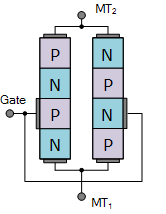
\includegraphics{img/triac1.png}
		\caption{Construcción física}%
		\label{fig:triac-construction}
	\end{subfigure}
	\begin{subfigure}{0.3\linewidth}
		\centering
		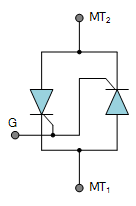
\includegraphics{img/triac2.png}
		\caption{Equivalente en tristores}%
		\label{fig:triac-analogy}
	\end{subfigure}
	\begin{subfigure}{0.3\linewidth}
		\centering
		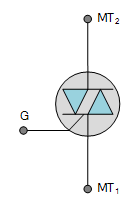
\includegraphics{img/triac3.png}
		\caption{Símbolo}%
		\label{fig:triac-symbol}
	\end{subfigure}
	\caption[Triac]{El Triac\footnotemark{}}%
		\label{fig:triac}
\end{figure}
\footnotetext{Fuente de imagen: \url{https://www.electronics-tutorials.ws/power/triac.html}}

Como siempre, al utilizar un TRIAC es deseable aislar la parte de corriente directa del circuito de la parte de corriente alterna, es decir, el TRIAC deberá estar aislado pero acoplado al circuito DC.
Esto normalmente se realiza mediante el uso de optoacopladores tipo MOC, tal como se ilustra en la \Cref{fig:triac-circuit}.

\begin{figure}[H]
	\centering
	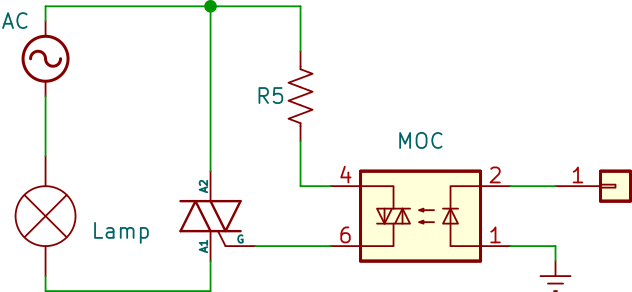
\includegraphics[width=0.5\textwidth,height=5cm,keepaspectratio]{img/triac-circuit.png}
	\caption{Triac optoacoplado}
	\label{fig:triac-circuit} %chktex 24
\end{figure}

Una peculiaridad de los TRIAC es que el tiempo de encendido no es proporcional al tiempo que se inyecta una corriente por el \emph{gate}, sino que una vez recibido el pulso de arranque el TRIAC permanecerá habilitado hasta el siguiente cruce por cero de la onda senoidal de corriente alterna.
Es decir que, diferencia de los transistores de juntura bipolar (BJT) o de efecto de campo (FET), un TRIAC no puede usarse para modular corriente directa con un PWM.
Por este motivo es necesario utilizar el \textbf{complemento} del ángulo de fase al modular la potencia de un dispositivo usando un TRIAC.

Por ejemplo, supóngase que se desea obtener el 50\% de potencia\footnotemark{} de una resistencia,
considerando que una resistencia tiene una respuesta lineal (el voltaje y la corriente están en fase) y que la senoidal de la línea de AC es una simétrica.
% el ángulo de disparo $\phi$ sería de $\phi = \frac{\pi}{2}$.

\begin{align*}
	% \frac{V_{P}}{2} = &
	% V_{P} \cdot \sin\left(2\pi \cdot f \cdot t\right) \\
	\cancel{V_{P}} = &
	\cancel{V_{P}} \cdot \sin\left(2\pi \cdot f \cdot t\right) \\%
	%
	1 = &
	\sin\left(2\pi \cdot f \cdot t\right) \\%
	%
	\arcsin\left(1\right) = &
	\cancel{\arcsin}\left(\cancel{\sin}\left(2\pi \cdot f \cdot t\right)\right) \\%
	%
	\frac{\pi}{2} = &
	2\pi \cdot f \cdot t\\%
	%
	t = &
	\frac{\frac{\cancel{\pi}}{2}}{2\cancel{\pi} \cdot f} \\%
	%
	t =& \frac{1}{4f}
\end{align*}

Si la frecuencia de línea fuera de 50Hz, el tiempo de disparo $t_{50\%}$ después del cruce por cero sería:

\begin{align*}
	t_{50\%} =& \frac{1}{4 \times 50\text{Hz}} \\
	=& \frac{1}{200\frac{1}{s}} \\
	=& 0.005s \\
	=& 5ms \\
\end{align*}

De acuerdo con lo anterior, el triac deberá encenderse en $t=5ms$ y así permanecerá encendido hasta que el voltaje de la línea pase por cero y se invierta, es decir, la mitad del ciclo.
Ni siquiera es necesario mantener la señal de encendido del TRIAC durante este tiempo.
Para encender el triac basta con un breve pulso normalmente despreciable (ej.~$10\mu s$).

% En contraste, si la señal de habilitación de se encendiera en $t=0$ y apagarse en $t=5ms$; sin embargo, tal como se mencionó anteriormente, si el TRIAC se enciende en $t=0$ éste permanecerá encendido durante todo el ciclo

\footnotetext{
	Como $P=VI$ y $V=RI$ entonces $P=\frac{V^{2}}{R}$ donde $V$ es el voltaje promedio o RMS suministrado.
	Aquí es necesario hacer una distinción entre el voltaje RMS nominal de línea $V_L$ y el voltaje RMS de la onda recortada por del TRIAC $V_\alpha$, pues la potencia suministrada se corresponderá con este último de la forma:
	\begin{equation}
	\label{eqn:va}
		V_\alpha = V_L\sqrt{
			\frac{1}{\pi}
			\left(
				\pi - \alpha +
				\frac{\sin\left(2\alpha\right)}{2}
			\right)
		}
		\text{ ; donde } \alpha=\omega t
		\text{ y } \omega = 2\pi f
	\end{equation}

	Cuando lo que interesa es un percentil de la potencia suministrada se tiene que
	$P_\text{\textsc{Max}} = P_L = P_{\alpha=0}$,
	por lo que se puede utilizar el cociente
	$\frac{P_\alpha}{P_L} = \frac{V_\alpha^{2}\cancel{R}}{V_L^{2}\cancel{R}}$ que, despejando en la \Cref{eqn:va} produce:

	\begin{equation}
	\label{eqn:pa}
		P\% = \left(
			1 - \frac{\alpha}{\pi} +
			\frac{\sin\left(2\alpha\right)}{2\pi}
		\right) \times 100
	\end{equation}

	Que, a una frecuencia de 50Hz y con $t=5ms$ ($\alpha=0.5\pi$) reporta un 50\% de potencia.

	Es importante remarcar que la \Cref{eqn:pa} es válida sólo si la impedancia de la carga es invariante en el tiempo ($\frac{dR}{dt}=0$).
	Si este no fuere el caso (como por ejemplo con una lámpara incandescente) la potencia no variará de forma cuadrática proporcional con el voltaje.
}


% %% %%%%%%%%%%%%%%%%%%%%%%%%%%%%%%%%%%%%%%%%%%%%%%%%%%%%%%%%%%
% intro-dimmer.tex
%
% Author:  Mauricio Matamoros
% License: MIT
%
% %% %%%%%%%%%%%%%%%%%%%%%%%%%%%%%%%%%%%%%%%%%%%%%%%%%%%%%%%%%%
%!TEX root = ../practica.tex
%!TEX root = ../references.bib

% CHKTEX-FILE 1
% CHKTEX-FILE 13
% CHKTEX-FILE 46

\subsection{Modulación de potencia de carga resistiva en AC}%
\label{seq:intro-dimmer}

A diferencia de un circuito de DC, la modulación de la potencia de una carga en un circuito de AC de una fase incolucra cuatro parámetros:
\begin{enumerate*}[label=\roman*\rpar]
	\item el voltaje en la carga,
	\item la corriente que circula por la carga,
	\item la impedancia de la carga
	y
	\item el ángulo de fase.
\end{enumerate*}
O, matemáticamente hablando:

\begin{align}
	p(t) & =vi
	\label{eq:pvi}\\
	  & =
		V_{m}\sin\left(\omega t + \theta_v \right)
		% \times
		I_{m}\sin\left(\omega t + \theta_i \right)
	\label{eq:pvi-full}
\end{align}

\noindent donde:

\begin{itemize}[noitemsep]
	\item $\omega$ la velocidad angular tal que $\omega = 2 \pi f$
	\item $V_{m}$ el voltaje máximo
	\item $I_{m}$ la corriente máxima
	\item $\theta_v$ el ángulo de fase del voltaje
	\item $\theta_i$ el ángulo de fase de la corriente
\end{itemize}

De estos cuatro parámetros, en un circuito puramente resistivo la impedancia $R$ es constante, la corriente $i(\omega t + \theta_i)$ es proporcional al voltaje a la entrada de la carga y a la resistencia de la misma, y el voltaje $v(\omega t + \theta_v)$ oscila en el rango $\left[-V_m, V_m\right]$, con $V_m$ el voltaje de pico.
No obstante, se puede modificar voltaje promedio en la carga al variar el ángulo de fase y así controlar la potencia.
Esta técnica es de hecho el principio fundamental de los circuitos convertidores de AC-AC a base de TRIAC como el que se muestra en la \Cref{fig:ac-ac-conv}.

\begin{figure}[H]
	\centering
	\begin{subfigure}[b]{0.5\columnwidth}
		\centering
		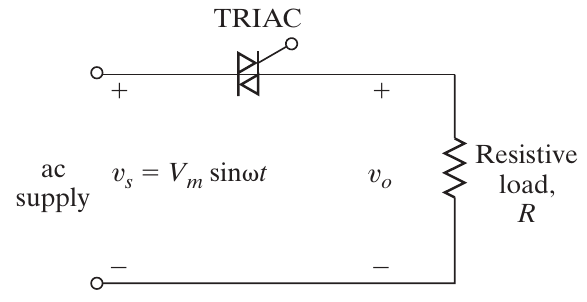
\includegraphics[width=\textwidth,height=3cm,keepaspectratio]{img/ac-ac-conv-dia.png}
		\caption{Circuito}%
		\label{fig:ac-ac-conv-dia} %chktex 24
	\end{subfigure}%
	\begin{subfigure}[b]{0.5\columnwidth}
		\centering
		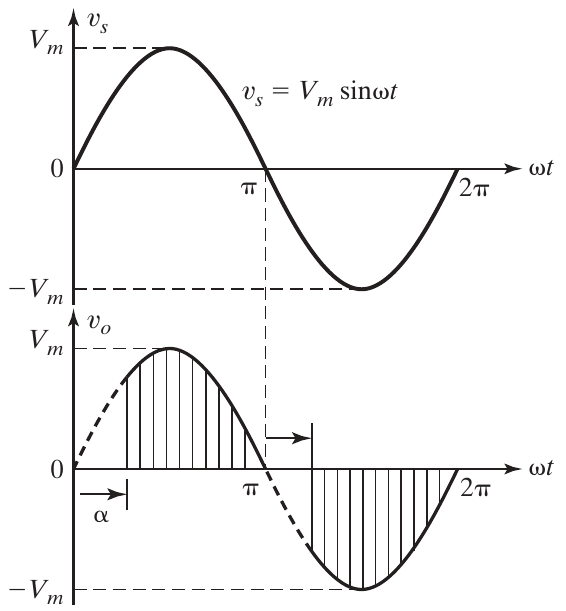
\includegraphics[width=\textwidth,height=5cm,keepaspectratio]{img/ac-ac-conv-wave.png}
		\caption{Señal voltaica}%
		\label{fig:ac-ac-conv-wave} %chktex 24
	\end{subfigure}
	\caption[Convertidor AC-AC]{Convertidor AC-AC de una fase.\footnotemark{}}%
	\label{fig:ac-ac-conv} % chktex 24
\end{figure}
\footnotetext{Fuente de la imagen: \Citet[pp.~33]{Rashid2006}.}

Nótese que los ángulos de defasamiento de voltaje $\theta_v$ y corriente $\theta_i$ han desaparecido.
Esto se debe a que en un circuito de AC de una sola fase $\theta_v = 0$ por ser la única fase y por ende la referencia.
Además, en un circuito puramente resistivo las señales de voltaje y corriente están acopladas, por lo que $\theta_i = \theta_v$ tal como se muestra en la \Cref{fig:ac-v-i}.

\begin{figure}[H]
% \begin{wrapfigure}{r}{0.3\columnwidth}
	\centering
	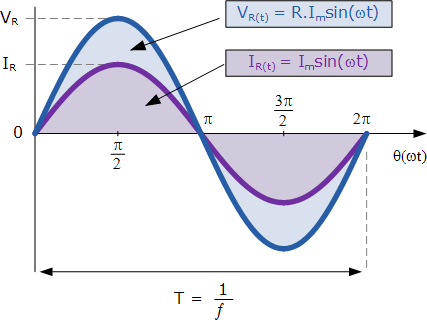
\includegraphics{img/ac-v-i.png}
	\caption[Voltaje y corriente en un circuito resistivo monofase]%
	{Voltaje y corriente en un circuito resistivo monofase.\footnotemark{}}%
	\label{fig:ac-v-i}
	\footnotetext{Fuente de imagen: \url{https://www.electronics-tutorials.ws/accircuits/ac-resistance.html}}
% \end{wrapfigure}
\end{figure}

En la mayoría de los casos lo que interesa no es el cálculo de la potencia neta, sino controlar el factor de potencia, el decir, el porcentaje de la potencia máxima que la carga está entregando.
Al estar sincronizadas la corriente y el voltaje por ser un circuito resistivo y no existir más que una fase, el cálculo de la potencia se simplifica y se convierte en el cociente del voltaje promedio aplicado a la carga respecto al voltaje RMS de la línea.
Es decir

\begin{align}
	P_f = \frac{V_o}{V_{RMS}}
	\label{eq:pf}
\end{align}

\noindent y dado que $V_{RMS}$ es fijo, lo que interesa calcular es el voltaje aplicado a la carga $V_o$ que se calcula como~\Citep[579--583]{Rashid2006}:%
\footnote{El valor medio o efectivo de cualquier función $f(\omega t)$ con periodo de $2\pi rad$ está determinado por
	$F = \sqrt{
		\frac{1}{2\pi}
		\int^{2\pi}_0
		f^2\left(\omega t\right) d\omega t
	}$
}

\begin{align}
	V^2_o = &
		\frac{2}{2\pi}
		\int^\pi_\alpha
		2V^2_{RMS}\sin^2\left(\omega t\right)
		d\left(\omega t\right)
		\\
	= &
		\frac{4V^2_{RMS}}{4\pi}
		\int^\pi_\alpha
		\big(1-\cos\left(2\omega t\right)\big)
		d\left(\omega t\right)
		\\
	= &
		\frac{V^2_{RMS}}{\pi}
		\left(
			\pi-\alpha + \frac{\sin\left(2\alpha\right)}{2}
		\right)
\end{align}

\noindent Por lo tanto

\begin{align}
	V_o = &
		{\left[
			\frac{V^2_{RMS}}{\pi}
			\left(
				\pi-\alpha + \frac{\sin\left(2\alpha\right)}{2}
			\right)
		\right]}^\frac{1}{2}
		\\
	=&
		V_{RMS}\sqrt{
		\frac{1}{\pi}
		\left(
			\pi-\alpha + \frac{\sin\left(2\alpha\right)}{2}
		\right)
		}
	\label{eq:po}
\end{align}

Ahora, supóngase que se desea modular la potencia de un foco incandescente de $60W$ conectado a una línea estándar de $V_{RMS}=120V$, 60Hz.
Como $P=\frac{V^2}{R}$ se puede calcular tanto la resistencia del foco como la corriente a fin de elegir el TRIAC adecuado:

\begin{align*}
	R =& \frac{V^2}{P} \\
	=&
		\frac{{\left(120V\right)}^2}{60W} \\
	=&
		\frac{14400V^2}{60W} \\
	=& 240\Omega
\end{align*}

\noindent y como $I=\frac{V}{R}$
\begin{align*}
	I_{RMS} & = \frac{120V}{240\Omega} = 0.5A\\
	I_{m} & = \sqrt{2} \times I_{RMS} =\sqrt{2} \times 0.5A\\
	      & = 0.7A
\end{align*}

\cleardoublepage
Ahora bien, si se usa un ángulo de disparo en el TRIAC de $\alpha = \frac{\pi}{2}$ la potencia de el foco con base en las \Cref{eq:pf,eq:po} será:

\begin{align*}
	P_f &= \frac{V_o}{V_{RMS}} \\
	&= \frac{\cancel{V_{RMS}}{~\left[
			\frac{1}{\pi}
			\left(
				\pi-\alpha + \frac{\sin\left(2\alpha\right)}{2}
			\right)
			\right]}^\frac{1}{2}
		}{\cancel{V_{RMS}}}
	\\
	&=
		{~\left[
			\frac{1}{\pi}
			\left(
				\cancelto{\frac{\pi}{2}}{\pi-\frac{\pi}{2}} +
				\frac{\sin\left(\frac{\cancel{2}\pi}{\cancel{2}}\right)}{2}
			\right)
		\right]}^\frac{1}{2}
	\\
	&=
		{\left[
			\frac{1}{\pi}
			\left(
				\frac{\pi}{2} +
				\cancelto{0}{\frac{\sin\left(\pi\right)}{2}}
			~~~\right)
		\right]}^\frac{1}{2}
	\\
	&=
		{\left(
			\frac{1}{\cancel{\pi}}
			\cdot
			\frac{\cancel{\pi}}{2}
		\right)}^\frac{1}{2}
	\\
	&= \sqrt{\frac{1}{2}}\\
	&= 0.707 \\
	&= 70.7\%
\end{align*}

De este desarrollo se concluye, además, que el factor de potencia no depende de los valores de voltaje, sino sólo del ángulo de disparo del TRIAC $\alpha$.

Como $\alpha = \omega t$, para conocer el tiempo de disparo $\tau$ basta con sustituir $t=\tau$ y despejar.
Así:

\begin{align*}
	\tau =& \frac{\alpha}{\omega} \\
	=&
		\frac{\alpha}{2 \pi f} \\
	=&
		\frac{\frac{\pi}{2}}{2 \pi f}\bigg\rvert_{f=60\text{Hz}}
		\\
	=&
		\frac{1}{4 \times 60\text{Hz}} =
		\frac{1}{240\text{Hz}}
		\\
	=& 0.00416\bar{6}\text{s} \\
	\approx& 4.2\text{ms}
\end{align*}

Un problema importante a considerar es que la ecuación
\(
	P_f = {~\left[
		\frac{1}{\pi}
		\left(
			\pi-\alpha + \frac{\sin\left(2\alpha\right)}{2}
		\right)
	\right]}^\frac{1}{2}
\)
no es biyectiva (tiene una componente periódica senoidal) y por lo tanto no es posible calcular su inversa de forma analítica.
En otras palabras, no es posible obtener una expresión algebraica para calcular $\alpha\left(P_f\right)$, y por tampoco es posible inferir $\tau\left(P_f\right)$.

Existen varias soluciones alterna a este problema.
Por ejemplo, pueden utilizarse varios métodos de aproximación numérica para cada uno de los segmentos de la curva y utilizar el más adecuado para en cada uno de los rangos de interés.
Otros métodos que requieren un número mucho menor de cálculos hacen uso de una tabla de valores discretos (por ejemplo incrementos de 1\% en el factor de potencia) e interpolan linealmente entre estos, dejando el error como una perturbación a corregir por el controlador (véase \Cref{tbl:trigger-time}).

\begin{table}[H]
	\centering
	\captionsetup{justification=centering,margin=2cm}
	\caption{Relación entre factor de potencia y tiempo de disparo de TRIAC\\Tabla para interpolación con incrementos de 5\% y alimentación de AC a 60Hz}%
	\label{tbl:trigger-time}
	\begin{tabular}{c c  c c  c c}
		\toprule
		\textbf{\small Factor de} &
		\textbf{\small Tiempo de} &
		\textbf{\small Factor de} &
		\textbf{\small Tiempo de} &
		\textbf{\small Factor de} &
		\textbf{\small Tiempo de}\\
		\textbf{\small potencia [\%]} &
		\textbf{\small disparo [ms]}  &
		\textbf{\small potencia [\%]} &
		\textbf{\small disparo [ms]}  &
		\textbf{\small potencia [\%]} &
		\textbf{\small disparo [ms]} \\
		\midrule
		100 & 0.000 &  65 & 4.464 &  30 & 6.232 \\
		 95 & 2.060 &  60 & 4.734 &  25 & 6.487 \\
		 90 & 2.696 &  55 & 4.993 &  20 & 6.750 \\
		 85 & 3.157 &  50 & 5.245 &  15 & 7.030 \\
		 80 & 3.538 &  45 & 5.493 &  10 & 7.334 \\
		 75 & 3.874 &  40 & 5.738 &   5 & 7.688 \\
		 70 & 4.179 &  35 & 5.984 &   0 & 8.203 \\
		\bottomrule
	\end{tabular}
\end{table}

% %% %%%%%%%%%%%%%%%%%%%%%%%%%%%%%%%%%%%%%%%%%%%%%%%%%%%%%%%%%%
% intro-i2c.tex
%
% Author:  Mauricio Matamoros
% License: MIT
%
% %% %%%%%%%%%%%%%%%%%%%%%%%%%%%%%%%%%%%%%%%%%%%%%%%%%%%%%%%%%%

%!TEX ROOT=../main.tex
%!TEX ROOT=../references.bib

% CHKTEX-FILE 1
% CHKTEX-FILE 46

\begin{wrapfigure}{r}{0.3\columnwidth}
	\centering
	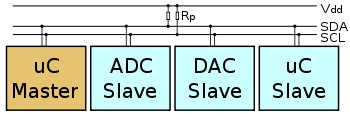
\includegraphics[width=0.3\columnwidth]{img/i2c-bus.png}
	\caption{Bus \IIC}%
	\label{fig:iic-bus}
\end{wrapfigure}
\IIC~es un protocolo serial inventado por Phillips y diseñado para conectar dispositivos de baja velocidad mediante interfaces de dos hilos (\Cref{fig:iic-bus}).
El protocolo permite un número virtualmente ilimitado de dispositivos interconectados donde más de uno puede ser un dispositivo maestro.
El bus I2C es popular debido a su facilidad de uso y fácil configuración.
Sólo es necesario definir la velocidad máxima del bus, que está conformado por dos cables con resistencias pull-up~\Citep{IICWeb}.

\IIC~utiliza solamente dos cables: SCL (reloj) y SDA (datos).
La transferencia de datos es serial y transmite paquetes de 8 bits con velocidades de hasta 5MHz.
Además, es requisito que cada dispositivo esclavo tenga una dirección de 7 bits que (el bit más significativo se utiliza para indicar si el paquete es una lectura o una escritura) debe ser única en el bus.
Los dispositivos maestros no necesitan dirección ya que estos generan la señal de reloj y coordinan a los dispositivos esclavos~\Citep{IICWeb}.

En \IIC~todas las operaciones son iniciadas por un dispositivo maestro que provee el reloj (se permiten múltiples maestros) e indica el tipo de operación junto con la dirección del esclavo en un sólo byte.
Si la operación es de lectura, el dispositivo maestro cambiará el pin SDA como entrada y escuchará la respuesta del dispositivo esclavo.
Si, por el contrario, la operación es de lectura, el dispositivo maestro enviará los datos vía SDA y esperará un bit de OK (0) como respuesta del dispositivo esclavo, leyendo un valor cero cuando el esclavo no contesta o hubo un error en la transmisión de datos.


